\chapter{Arhitektura i dizajn sustava}
		
		\textbf{\textit{dio 1. revizije}}\\

		\textit{ Potrebno je opisati stil arhitekture te identificirati: podsustave, preslikavanje na radnu platformu, spremišta podataka, mrežne protokole, globalni upravljački tok i sklopovsko-programske zahtjeve. Po točkama razraditi i popratiti odgovarajućim skicama:}
	\begin{itemize}
		\item 	\textit{izbor arhitekture temeljem principa oblikovanja pokazanih na predavanjima (objasniti zašto ste baš odabrali takvu arhitekturu)}
		\item 	\textit{organizaciju sustava s najviše razine apstrakcije (npr. klijent-poslužitelj, baza podataka, datotečni sustav, grafičko sučelje)}
		\item 	\textit{organizaciju aplikacije (npr. slojevi frontend i backend, MVC arhitektura) }		
	\end{itemize}

	
		

		

				
		\section{Baza podataka}
			
			\textbf{\textit{dio 1. revizije}}\\
			
		\textit{Za potrebe našeg sustava koristit ćemo relacijsku bazu podataka koja svojom strukturom olakšava modeliranje stvarnog svijeta. Gradivna jedinka baze je relacija, odnosno tablica koja je definirana svojim imenom i skupom atributa. Zadaća baze podataka je brza i jednostavna pohrana, izmjena i dohvat podataka za daljnju obradu. Baza podataka ove aplikacije sastoji se od sljedećih entiteta:}
		\begin{packed_item}
			\item Korisnik
			\item Sudionik
			\item Animator
			\item Organizator
			\item Prijava
			\item Grupa
			\item Raspored
			\item Sjednica
			\item Aktivnost
			\item Kamp
			\item Animator\_ocjena\_aktivnosti
			\item Sudionik\_ocjena\_aktivnosti
		\end{packed_item}
			\subsection{Opis tablica}
			

				\textit{\textbf{Korisnik}	Ovaj entitet sadržava sve važne informacije o korisniku aplikacije. Sadrži atribute: korisnicko\_ime, lozinka, email, ime, prezime, status. Ovaj entitet u vezi je One-to-One s entitetom Sudionik preko atributa korisnicko\_ime, u vezi One-to-One s entitetom Animator preko atributa korisnicko\_ime, u vezi One-to-One s entitetom Organizator preko atributa korisnicko\_ime, te u vezi One-to-One s entitetom Prijava preko atributa korisnicko\_ime.}
				
				\begin{longtabu} to \textwidth {|X[6, l]|X[6, l]|X[20, l]|}
					
					\hline \multicolumn{3}{|c|}{\textbf{Korisnik }}	 \\[3pt] \hline
					\endfirsthead
					
					\hline \multicolumn{3}{|c|}{\textbf{Korisnik}}	 \\[3pt] \hline
					\endhead
					
					\hline 
					\endlastfoot
					
					\cellcolor{LightGreen}Korisnicko ime & VARCHAR	& jedinstveni identifikator korisnika\\ \hline
					Lozinka	& VARCHAR & lozinka korisnika	\\ \hline 
					Email & VARCHAR &  email korisnika \\ \hline 
					Ime & VARCHAR	&  ime korisnika		\\ \hline 
					Prezime & VARCHAR	& prezime korisnika 		\\ \hline 
					Status & VARCHAR	& status korisnika(status prijave?) 		\\ \hline 
					
					
				\end{longtabu}
			
				\textit{\textbf{Sudionik}	Ovaj entitet sadržava sve važne informacije vezane za sudionika u kampu. Sadrži atribute: korisnicko\_ime\_sudionik, br\_tel\_sudionik, datum\_i\_god\_rod\_sudionik, br\_tel\_odg\_osobe, motivacijsko\_pismo\_sudionik, id\_grupa. Ovaj entitet je u One-to-Many vezi s entitetom Sudionik\_ocjena\_aktivnosti preko atributa korisnicko\_ime\_sudionik, u vezi Many-to-one s entitetom Grupa preko atributa id\_grupa, te u vezi One-to-One  s entitetom Korisnik preko atributa korisnicko\_ime\_sudionik.}
				
				\begin{longtabu} to \textwidth {|X[6, l]|X[6, l]|X[20, l]|}
					
					\hline \multicolumn{3}{|c|}{\textbf{Sudionik}}	 \\[3pt] \hline
					\endfirsthead
					
					\hline \multicolumn{3}{|c|}{\textbf{Sudionik}}	 \\[3pt] \hline
					\endhead
					
					\hline 
					\endlastfoot
					
					\cellcolor{LightGreen}Korisnicko ime sudionik & VARCHAR	&  jedinstveni identifikator korisnika( sudionika) 	\\ \hline
					Br tel sudionik	& INT & broj telefona sudionika   	\\ \hline 
					Datum i god rod sudionik & DATE & datum i godina rođenja sudionika  \\ \hline 
					Br tel odg osobe & INT	&  broj telefona odgovorne osobe( ako je sudionik mlađi od 18)		\\ \hline
					Motivacijsko pismo sudionik & VARCHAR	&  motivacijsko pismo sudionika		\\ \hline 
					\cellcolor{LightBlue} ID grupa	& INT & jedinstveni identifikator grupe sudionika  	\\ \hline 
					
					
				\end{longtabu}
			
				\textit{\textbf{Animator}	Ovaj entitet sadržava sve važne informacije vezane za animatora u kampu. Sadrži atribute: korisnicko\_ime\_animator, br\_tel\_animator, datum\_i\_god\_rod\_animator, motivacijsko\_pismo\_animator. Ovaj entitet je u One-to-One vezi s entitetom Korisnik preko atributa korisnicko\_ime\_animatora, u vezi Many-to-One s entitetom Raspored preko atributa korisnicko\_ime\_animator, te u vezi One-to-Many s entitetom Animator\_ocjena\_aktivnosti preko atributa korisnicko\_ime\_animator.}
				
				\begin{longtabu} to \textwidth {|X[6, l]|X[6, l]|X[20, l]|}
					
					\hline \multicolumn{3}{|c|}{\textbf{Animator}}	 \\[3pt] \hline
					\endfirsthead
					
					\hline \multicolumn{3}{|c|}{\textbf{Animator}}	 \\[3pt] \hline
					\endhead
					
					\hline 
					\endlastfoot
					
					\cellcolor{LightGreen}Korisnicko ime animator & VARCHAR	&  jedinstveni identifikator korisnika( animatora)	\\ \hline
					Br tel animator	& INT &  broj telefona animatora 	\\ \hline 
					Datum i god rod animator & DATE & datum i godina rođenja animatora   \\ \hline 
					Motivacijsko pismo animator & VARCHAR	& motivacijsko pismo animatora 		\\ \hline 
					
					
				\end{longtabu}
			
				\textit{\textbf{Organizator}	Ovaj entitet sadrži sve važne informacije vezane za organizatora kampa. Sadrži atribut: korisnicko\_ime\_organizator. Ovaj entitet je u One-to-One vezi s entitetom Korisnik preko atributa korisnicko\_ime\_organizator.}
				
				\begin{longtabu} to \textwidth {|X[6, l]|X[6, l]|X[20, l]|}
					
					\hline \multicolumn{3}{|c|}{\textbf{Organizator}}	 \\[3pt] \hline
					\endfirsthead
					
					\hline \multicolumn{3}{|c|}{\textbf{Organizator}}	 \\[3pt] \hline
					\endhead
					
					\hline 
					\endlastfoot
					
					\cellcolor{LightGreen}Korisnicko ime organizator & VARCHAR	& jedinstveni identifikator korisnika( organizatora)	\\ \hline
				
					
					
				\end{longtabu}
			
				\textit{\textbf{Prijava}	Ovaj entitet sadrži sve važne informacije vezane o prijavama na kamp. Sadrži atribute: id\_prijava, korisnicko\_ime, datum\_i\_vrijeme\_prijave, status\_prijava. Ovaj entitet je u One-to-One vezi s entitetom Korisnik preko atributa korisnicko\_ime.}
				
				\begin{longtabu} to \textwidth {|X[6, l]|X[6, l]|X[20, l]|}
					
					\hline \multicolumn{3}{|c|}{\textbf{Prijava}}	 \\[3pt] \hline
					\endfirsthead
					
					\hline \multicolumn{3}{|c|}{\textbf{Prijava}}	 \\[3pt] \hline
					\endhead
					
					\hline 
					\endlastfoot
					
					\cellcolor{LightGreen}ID prijava & INT	& jedinstveni identifikator prijave  	\\ \hline
					\cellcolor{LightBlue}Korisnicko ime	& VARCHAR & jedinstveni identifikator korisnika  	\\ \hline 
					Datum i vrijeme prijava & DATETIME &  datum i vrijeme prijave \\ \hline 
					Status prijava & BOOLEAN	&  status prijave		\\ \hline 
					
					
				\end{longtabu}
			
				\textit{\textbf{Grupa}	Ovaj entitet sadrži sve važne informacije o grupama na kampu. Sadrži atribute: id\_grupa, ime\_grupa. Ovaj entitet je u One-to-Many vezi s entitetom Sudionik preko atributa id\_grupa, te u vezi Many-to-One s entitetom Raspored preko atributa id\_grupa.}
				
				\begin{longtabu} to \textwidth {|X[6, l]|X[6, l]|X[20, l]|}
					
					\hline \multicolumn{3}{|c|}{\textbf{Grupa}}	 \\[3pt] \hline
					\endfirsthead
					
					\hline \multicolumn{3}{|c|}{\textbf{Grupa}}	 \\[3pt] \hline
					\endhead
					
					\hline 
					\endlastfoot
					
					\cellcolor{LightGreen}ID grupa & INT	& jedinstveni identifikator grupe 		\\ \hline
					Ime grupa	& VARCHAR & ime grupe   	\\ \hline 
					
				\end{longtabu}
			
				\textit{\textbf{Raspored}	Ovaj entitet sadrži sve važne informacije vezane za raspored kampa. Sadrži atribute: id\_grupa, id\_aktivnost, datum\_i\_vrijeme\_izvrsavanja, korisnicko\_ime\_animator. Ovaj entitet je u One-to-Many vezi s entitetom Grupa preko atributa id\_grupa, Many-to-Many vezi s entitetom Animator preko atributa korisnicko\_ime\_animator, te u vezi One-to-Many s entitetom Aktivnost preko atributa id\_aktivnost.   }
				
				\begin{longtabu} to \textwidth {|X[6, l]|X[6, l]|X[20, l]|}
					
					\hline \multicolumn{3}{|c|}{\textbf{Raspored}}	 \\[3pt] \hline
					\endfirsthead
					
					\hline \multicolumn{3}{|c|}{\textbf{Raspored}}	 \\[3pt] \hline
					\endhead
					
					\hline 
					\endlastfoot
					
					\cellcolor{LightGreen}ID grupa & INT	&  jedinstveni identifikator grupe	\\ \hline
					\cellcolor{LightGreen}ID aktivnost	& INT & jedinstveni identifikator aktivnosti  	\\ \hline 
					\cellcolor{LightGreen}Datum i vrijeme izvrsavanja & DATETIME & datum i vrijeme izvršavanja    \\ \hline 
					\cellcolor{LightBlue}Korisnicko ime animator & VARCHAR	&  jedinstveni identifikator korisnika( animator)	\\ \hline 
					
					
					
				\end{longtabu}
			
				\textit{\textbf{Sjednica}	Ovaj entitet sadrži sve važne informacije o sjednici. Sadrži atribute: id\_sjednica, podatci, rok\_trajanja.}
				
				\begin{longtabu} to \textwidth {|X[6, l]|X[6, l]|X[20, l]|}
					
					\hline \multicolumn{3}{|c|}{\textbf{Sjednica}}	 \\[3pt] \hline
					\endfirsthead
					
					\hline \multicolumn{3}{|c|}{\textbf{Sjednica}}	 \\[3pt] \hline
					\endhead
					
					\hline 
					\endlastfoot
					
					ID sjednica & INT	& jedinstveni identifikator sjednice 	\\ \hline
					Podatci	& VARCHAR & podatci o sjednici  	\\ \hline 
					Rok trajanja & DATETIME & rok trajanja sjednice  \\ \hline 
					
					
				\end{longtabu}
			
				\textit{\textbf{Aktivnost}	Ovaj entitet sadrži sve važne o informacijama vezane za aktivnosti na kampu. Sadrži atribute: id\_aktivnost, ime\_aktivnost, opis\_aktivnost, trajanje\_aktivnost\_(sat/i), tip\_aktivnosti, datum\_odrzavanja\_kamp, ime\_kamp. Ovaj entitet je u One-to-Many vezi s entitetom Sudionik\_ocjena\_aktivnosti preko atributa id\_aktivnost, u Many-to-Many vezi s entitetom Kamp preko atributa ime\_kamp, u One-to-Many vezi s entitetom Animator\_ocjena\_aktivnosti preko atributa id\_aktivnosti te u Many-to-One vezi s entitetom Raspored preko atributa id\_aktivnost.}
				
				\begin{longtabu} to \textwidth {|X[6, l]|X[6, l]|X[20, l]|}
					
					\hline \multicolumn{3}{|c|}{\textbf{Aktivnost}}	 \\[3pt] \hline
					\endfirsthead
					
					\hline \multicolumn{3}{|c|}{\textbf{Aktivnost}}	 \\[3pt] \hline
					\endhead
					
					\hline 
					\endlastfoot
					
					\cellcolor{LightGreen}ID aktivnost & INT	& jedinstveni identifikator aktivnosti  	\\ \hline
					Ime aktivnost	& VARCHAR &  ime aktivnosti 	\\ \hline 
					Opis aktivnost & VARCHAR & opis aktivnosti  \\ \hline 
					Trajanje aktivnost (sat/i) & DECIMAL	& trajanje aktivnosti 		\\ \hline
					Tip aktivnost & VARCHAR	& tip aktivnosti  		\\ \hline 
					Datum odrzavanja kamp & DATE	&  datum održavanja kampa		\\ \hline 
					\cellcolor{LightBlue} Ime kamp	& VARCHAR &  ime kampa 	\\ \hline 
					
					
				\end{longtabu}
			
				\textit{\textbf{Kamp}	Ovaj entitet sadrži sve važne informacije o kampu. Sadrži atribute: ime\_kamp, datum\_odrzavanja\_kamp, trajanje\_(dan/a), pocetak\_prijava\_sudionika, kraj\_prijava\_sudionika, pocetak\_prijava\_animatora, kraj\_prijava\_animatora, broj\_grupa. Ovaj entitet je u Many-to-Many vezi s entitetom Aktivnost preko atributa ime\_kamp. }
				
				\begin{longtabu} to \textwidth {|X[6, l]|X[6, l]|X[20, l]|}
					
					\hline \multicolumn{3}{|c|}{\textbf{Kamp}}	 \\[3pt] \hline
					\endfirsthead
					
					\hline \multicolumn{3}{|c|}{\textbf{Kamp}}	 \\[3pt] \hline
					\endhead
					
					\hline 
					\endlastfoot
					
					\cellcolor{LightGreen}Ime kamp & VARCHAR	&  ime kampa	\\ \hline
					\cellcolor{LightGreen}Datum odrzavanja kamp & DATE	& datum održavanja kampa 	\\ \hline
					Trajanje (dan/a)	& INT & trajanje kampa  	\\ \hline 
					Pocetak prijava sudionika & DATETIME & datum i vrijeme početka prijave sudionika  \\ \hline 
					Kraj prijava sudionika& DATETIME	& datum i vrijeme  kraja prijave sudionika	\\ \hline 
					Pocetak prijava animatora& DATETIME	& datum i vrijeme pocetka prijava animatora 		\\ \hline 
					Kraj prijava animatora & DATETIME& datum i vrijeme kraja prijava animatora 		\\ \hline 
					Broj grupa & INT	& broj grupa 		\\ \hline 
					
					
				\end{longtabu}
			
				\textit{\textbf{Animator\_ocjena\_aktivnosti}	Ovaj entitet sadrži sve važne informacije o ocjenama aktivnosti sa strane animatora. Sadrži atribute: korisnicko\_ime\_animator. ocjena\_animator, dojam\_animator, id\_aktivnost. Ovaj entitet je u Many-to-one vezi s entitetom Animator preko atributa korisnicko\_ime\_animator, te u Many-to-One vezi s entitetom Aktivnost preko atributa id\_aktivnost.   }
				
				\begin{longtabu} to \textwidth {|X[6, l]|X[6, l]|X[20, l]|}
					
					\hline \multicolumn{3}{|c|}{\textbf{Animator\_ocjena\_aktivnosti}}	 \\[3pt] \hline
					\endfirsthead
					
					\hline \multicolumn{3}{|c|}{\textbf{Animator\_ocjena\_aktivnosti}}	 \\[3pt] \hline
					\endhead
					
					\hline 
					\endlastfoot
					
					\cellcolor{LightGreen}Korisnicko ime animator & VARCHAR	& jedinstveni identifikator korisnika( animator)	\\ \hline
					Ocjena animator	& INT & animatorova ocjena aktivnosti  	\\ \hline 
					Dojam animator & VARCHAR & animatorov dojam aktivnosti   \\ \hline 
					\cellcolor{LightBlue}ID aktivnost	& INT & jedinstveni identifikator aktivnosti	\\ \hline 
					
					
				\end{longtabu}
			
				\textit{\textbf{Sudionik\_ocjena\_aktivnosti}	Ovaj entitet sadrži sve važne informacije o ocjenama aktivnosti sa strane animatora. Sadrži atribute: korisnicko\_ime\_sudionik, ocjena\_sudionik, dojam\_sudionik, id\_aktivnost. Ovaj entitet je u Many-to-One vezi s entitetom Sudionik preko atributa korisnicko\_ime\_sudionik, te u Many-to-One vezi s entitetom Aktivnost preko atributa id\_aktivnost.}
				
				\begin{longtabu} to \textwidth {|X[6, l]|X[6, l]|X[20, l]|}
					
					\hline \multicolumn{3}{|c|}{\textbf{Sudionik\_ocjena\_aktivnosti}}	 \\[3pt] \hline
					\endfirsthead
					
					\hline \multicolumn{3}{|c|}{\textbf{Sudionik\_ocjena\_aktivnosti}}	 \\[3pt] \hline
					\endhead
					
					\hline 
					\endlastfoot
					
					\cellcolor{LightGreen}Korisnicko ime sudionik & VARCHAR	& korisnicko ime korisnika( sudionik) 	\\ \hline
					Ocjena sudionik	& INT & ocjena aktivnosti sudionika   	\\ \hline 
					Dojam sudionik & VARCHAR & dojam aktivnosti sudionika  \\ \hline 
					\cellcolor{LightBlue} ID aktivnost	& INT & jedinstveni identifikator aktivnosti  	\\ \hline 
					
					
				\end{longtabu}
			
			\eject
			
			
			\subsection{Dijagram baze podataka}
				\begin{figure}[H]
				\centerline{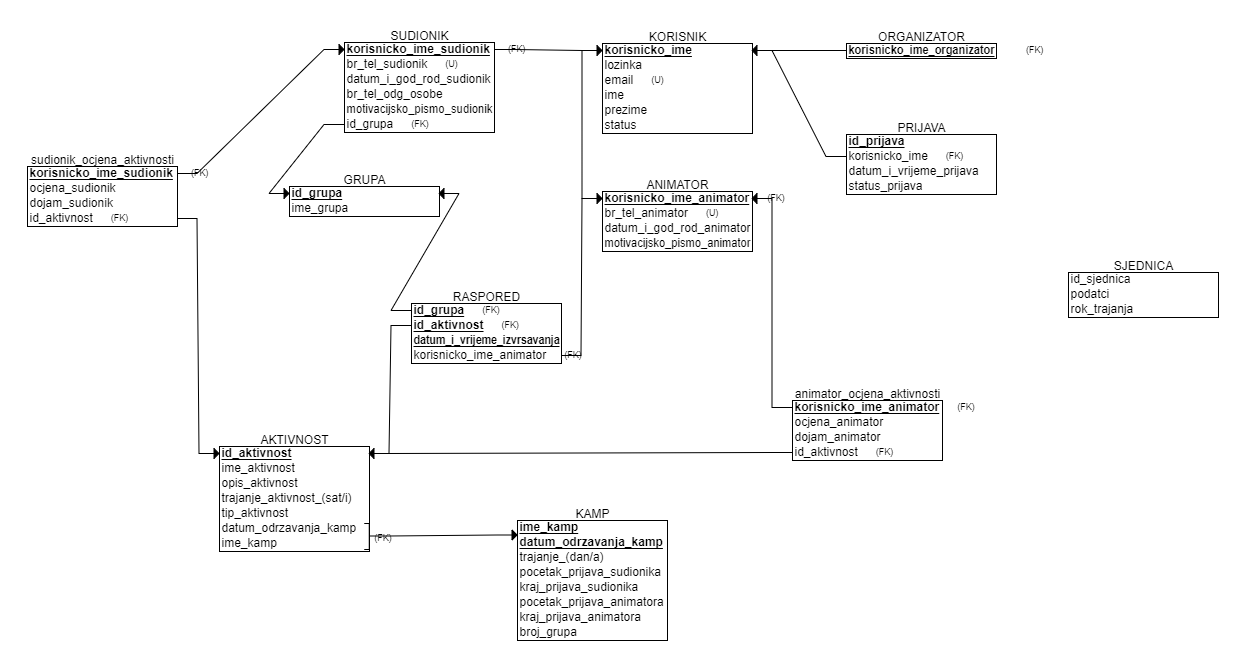
\includegraphics[width=\linewidth]{slike/ER_model_baze.png}}
				\caption{E-R dijagram baze podataka}
				\label{fig:ERdijagram}
			\end{figure}
			
			\eject
			
			
		\section{Dijagram razreda}
		
			\textit{Potrebno je priložiti dijagram razreda s pripadajućim opisom. Zbog preglednosti je moguće dijagram razlomiti na više njih, ali moraju biti grupirani prema sličnim razinama apstrakcije i srodnim funkcionalnostima.}\\
			
			\textbf{\textit{dio 1. revizije}}\\
			
			\textit{Prilikom prve predaje projekta, potrebno je priložiti potpuno razrađen dijagram razreda vezan uz \textbf{generičku funkcionalnost} sustava. Ostale funkcionalnosti trebaju biti idejno razrađene u dijagramu sa sljedećim komponentama: nazivi razreda, nazivi metoda i vrste pristupa metodama (npr. javni, zaštićeni), nazivi atributa razreda, veze i odnosi između razreda.}\\
			
			\textbf{\textit{dio 2. revizije}}\\			
			
			\textit{Prilikom druge predaje projekta dijagram razreda i opisi moraju odgovarati stvarnom stanju implementacije}
			
			
			
			\eject
		
		\section{Dijagram stanja}
			
			
			\textbf{\textit{dio 2. revizije}}\\
			
			\textit{Potrebno je priložiti dijagram stanja i opisati ga. Dovoljan je jedan dijagram stanja koji prikazuje \textbf{značajan dio funkcionalnosti} sustava. Na primjer, stanja korisničkog sučelja i tijek korištenja neke ključne funkcionalnosti jesu značajan dio sustava, a registracija i prijava nisu. }
			
			
			\eject 
		
		\section{Dijagram aktivnosti}
			
			\textbf{\textit{dio 2. revizije}}\\
			
			 \textit{Potrebno je priložiti dijagram aktivnosti s pripadajućim opisom. Dijagram aktivnosti treba prikazivati značajan dio sustava.}
			
			\eject
		\section{Dijagram komponenti}
		
			\textbf{\textit{dio 2. revizije}}\\
		
			 \textit{Potrebno je priložiti dijagram komponenti s pripadajućim opisom. Dijagram komponenti treba prikazivati strukturu cijele aplikacije.}